When reviewing the literature for this project, the available information fell into two categories:
on one hand, it was important to consult papers describing past attempts at classifying coffee beans,
especially those that proposed methods for doing it at scale.
On the other hand, looking at the wider world of image classification revealed useful details and approaches to
classifier architecture that informed the decisions made in this project.
Overall, considering the history of image classification as a field and its applications in the coffee industry
built the information background that enabled the development of the prototypes in this project.

\section{An overview of image classification algorithms}
\label{sec:lit-review-general}
The topic of image classification is one of the most researched and explored topics in the field of artificial intelligence.
Over the years, several approaches to image classification have been proposed, with each tailored to perform best with
certain kinds of images, sizes of datasets or hardware capabilities.

On the simpler side of image classification algorithms lies an application of a KNN classifier~\cite{knnOverview}, a method of
unsupervised learning, where the classifier ``learns'' from the differences between the datapoints rather than their labels.
A KNN classifier's main benefit is the lack of training time: instead, the images are compared to the others as soon as
they are available.
This allows for rapid prototyping and a quick implementation time at the cost of the resources needed to make each decision
when running the model.
Despite this tradeoff, versions of the KNN architecture remain a popular choice for image classification to this day,
and, with some modification, solve the large resource requirements by utilising advanced data structures, such as in the
case of the KN-KNN algorithm \cite{kdtreeKNN}.

Since the algorithm requires the calculation of ``distance'' between any given datapoints, several metrics of calculation
exist, such as Euclidean, Manhatan and more.
The choice of the distance metric as well as the value of K must be picked experimentally, with a technique such as
cross validation.
Overall, the KNN algorithm provides a quick and efficient way of prototyping an image classifier, however the simplicity
comes at a cost of the need to manually pick the necessary hyperparameters to get the best out of the architecture.


A more modern and complex solution can be found in neural networks.
These classifiers attempt to mimic the human neuron, where each neuron activates or ``fires'' only if some condition
(the ``activation function'') passes a certain threshold.

Neural networks can be used for more than image classification and are an actively developing topic to this day, however
some network architectures are known for their performance with images and are commonly used as the baseline for more domain
specific applications.
Some examples of such architectures include LeNet~\cite{leNetOverview} and AlexNet~\cite{alexNetOverview}, which are often
used for datasets containing smaller (in terms of pixel resolution) images, making them a good potential starting point
for use in this project.
AlexNet in particular has shown great potential with image datasets, such as CIFAR-10~\cite{cifar10}, which, given that
the number of roasted coffee defects roughly matches the number of classes in the CIFAR-10 dataset, suggests that an architecture
similar to AlexNet may be a good candidate for this project.

Unlike KNN classifiers, neural networks require significantly larger datasets as well as training time to fit the model
to the data at hand.
In exchange for the increased training time, neural networks boast a much faster classification time, with some even allowing
real-time classification.
While not explicitly a goal of this project, the potentially faster classification time would make a neural network-based
prototype a better fit for use in industry, allowing the classifier to be used at scale.

Data normalization is an important point to consider when using image classifiers.
For best performance, the images must be of similar dimensions and free of background noise or obstructions.
Therefore, when gathering data for this project, a significant amount of effort must be put into ensuring that each bean
is well-lit, on a clear background and that other beans do not protrude into the image.

The following section will contain a deeper look at previous attempts of classifying roasted coffee beans with KNN
as well as more complex, neural network based models.

\section{Coffee bean classification}
\label{sec:lit-review-coffee}
The overall picture gathered from reviewing the literature under this topic suggests that identifying
items as small as coffee beans is definitely possible, although not without some degree of effort invested in the process.
Several of the reviewed papers claimed great results, though for many, the data gathering and cleaning process involved
rare or expensive equipment.

An example of such study has been conducted by Chen et al. \cite{hyperspectralChen}, who have achieved an accuracy of
98.6\% when classifying green coffee beans.
While the purpose of their paper is slightly different, focusing on optimising a different stage in the coffee supply chain,
their approach to data collection and processing provided valuable insights serving as a great starting point.
Similar to this project, the authors have identified several green coffee defects to classify: insect damage,
black beans (ones that have prematurely fallen off the tree and could not develop) and bean fragments.

The images were taken in batches, using a hyperspectral scanner,
which captures light beyond the visible frequency range.
The paper's main strengths were in its design of the image processing pipeline and classifier architecture.
The capturing of images was automated using a conveyor belt feeding rows of beans of the same category under the scanner.
While the extra equipment required for this approach introduces extra costs and may be better fit for a commercial application,
the technique of splitting an image of a row of beans into groups of individual images,
all resized to the same dimensions provided a great way to simplify and speed up the data gathering process for this project.

The authors, using neural networks to classify the images, have provided several classifier architectures.
While the highest-performing network in their study (a 3D-CNN) required leveraging the hyperspectral data provided by the scanner,
the 2D-CNN architecture they described used only the spatial data of the images.
Interestingly, the CNN-based classifiers boasted fast classification time, with the authors developing a real-time sorting device.
While physical prototypes are beyond the scope of this project, knowing that near real-time classification speeds are
possible with this architecture suggests that this approach could fit the task at hand well.
Furthermore, Chen et al.\ employed a dimensionality reduction algorithm (PCA) for their model, which has improved the overall accuracy
when reducing the hyperspectral data down to 3 components.
This increase in performance could also be investigated and leveraged in this project.

Despite the high performance and large dataset in Chen et al.'s paper, the real-world performance of any model could
be improved by a more diverse dataset, showing either more defects, more coffee varieties, or both.
This project aims to cover this gap by utilising beans processed by various methods, from several distinct origins and species.

Oliveri et al.\  take a slightly different approach in their 2019 paper \cite{hyperspectralGreenOliveri}.
Rather than utilising a deep learning network, they instead used a K-nearest-neighbour (KNN) classifier to assign the closest
category to a given bean image.
Similar to the previous paper, the authors have identified three classes of bean defects, however the defects were slightly different:
instead of insect damage, the authors instead focused on beans that have lost too much moisture.
THe data gathering process was similar to that of Chen et al., as was their use of PCA to extract the key components
to be used for classification.

The authors did not develop any physical apparatus to separate the defective beans in their paper, however
they were able to process images of groups of beans, highlighting defective ones on the original image.
This approach fits really well with the constraints and aims of this project, as being able to identify defects and
determine their place on the original image would already lead to a significant saving of effort and time for the potential users.

Another strength of Oliveri et al's paper is in their iterative and transparent approach to the development of the model.
The authors were one of the few who mentioned cross validation as part of their project and explained the choice of the number
of neighbours for their classifier.
Furthermore, they admitted that due to the rarity of certain bean defects, they were not able to gather enough samples
to add them to the classifier as well as having to remove a number of beans from the sample pool to make the ratio of beans
in each class as even as possible.

While the above shortcoming, coupled with a lack of reporting on the species or processing of the beans, identifies areas for
improvement, the overall approach shows great potential in identifying defects.
The application of the model and its design have influenced the research process for this project, which,
with a more varied dataset, aims to explore the topic of KNN classification further.

A 2017 paper by Nasution and Andayani~\cite{manyRoastLevelsNasution} shows a departure from the previous two paper both
in its approach to data gathering as well as the overall aim.
Instead of focusing on green coffee defects, they instead focused on coffee roast levels, aiming to classify the beans'
degree of roast on a scale of 16 levels, from completely green to burnt.
The images were gathered using a common smartphone camera and resized to the same dimensions,
with each image containing a single bean.
For their classifier, the authors chose a backpropagation neural network, with the images first processed by a
gray level co-occurrence matrix (GLCM), a technique that allows to develop insights into textures of surfaces from an image.

Overall, the authors claim an accuracy of 97.5\%, however the report lacks transparency in the total number of samples
as well as the way classes were determined, with some roast levels only having a slight difference in hue.
With such a fine-grained scale of roast levels, it is difficult to see how the authors were able to find a sufficient
quantity of beans at each level and classify them without samples of one class mixing into others.
Despite this lack of transparency, the paper still provides a valuable look at how a task similar to the one in this project
can be done without requiring complex and expensive equipment.
The results achieved by the paper, while being able to benefit from more clarity in reporting, suggest the possibility of
developing a classifier that:
\begin{itemize}
    \item Is able to work on visible-light images only
    \item Is able to pick up on small changes in the surface of the beans
    \item Differentiates roasted beans, which may have less colour variation than green beans with a similar degree of accuracy
\end{itemize}

\begin{wrapfigure}{r}{0.5\textwidth}
    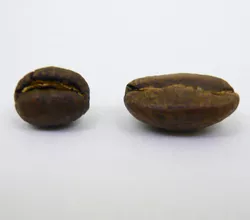
\includegraphics[width=0.5\textwidth]{figures/litReview/peaberry-vs-normal}
    \caption*{Source: \cite{peaberryImg}}
    \caption{An example of a ``peaberry'' coffee bean (left)}
    \caption*{Note the smaller size and round shape.}
    \label{fig:peaberryComparison}
\end{wrapfigure}
A paper with one of the closest aims to this project was written by Shao et al.\ in 2022\cite{rgbDeepLearningShao}.
Similar to this project, the paper aims to classify roasted beans, with the authors identifying a similar number of bean defects.
Interestingly, the authors identify ``peaberry'' beans or beans with an exceptionally small, round shape as seen on figure \ref{fig:peaberryComparison},
as a defect, whereas many coffee consumers and producers believe that such beans provide a flavour advantage over regular beans
and market them as the more desirable species.
It should be noted that this paper highlights the usefulness of automated bean classification: with a sufficiently well-trained
model, a physical prototype could be implemented to sort the beans, allowing the producers to discard or separate the bean
classes they deem valuable or defective.
In that regard, Shao et al's paper is an important showcase of the economic benefits brought along by automatization
of the coffee quality control process.

The authors have also provided an automated method of data gathering, utilizing a rotating wheel to briefly hold the beans
in front of a camera.
Similar to Nasution et al.\cite{manyRoastLevelsNasution}, the authors worked with RGB images and did not employ any
light spectra beyond the visible one.

The authors have used an existing, well-researched CNN architecture to develop their model, with 11 total layers,
achieving an accuracy as high as 96\% with the lowest score of 88\% across the seven identified classes.
Similar to commercial solutions described in section \ref{sec:qc-state-of-the-art}, the authors have used an air compressor
to automatically remove defective beans, proposing a lower-cost, more customizable solution of coffee quality control.

While the authors did not make any mention of the number of beans of each category they gathered or the breakdown of origins
and processing methods of the beans, the high total number (1700) of the beans suggest that there was sufficient data to train the model.
A potential improvement could be seen in a more varied dataset with a more even breakdown of classes.

Apart from the described usage of expensive and complex machinery to automatically gather the images and remove the defective beans,
the approach taken by Shao et al.\ showcases a low-cost approach, requiring only a visible-light camera and
sufficiently powerful hardware to train the model.

While gathering data for a prototype project is a relatively straightforward task, a real-life coffee roaster may have
access to a much greater number of defects and may be in search of a more resilient solution that requires less manual interaction
compared to manually laying the beans out to take images of them.
A possible solution to this problem can be seen in a 2024 paper by Eron et al. \cite{eronCoffeeCherryOnTrees}, proposing
the use of image classifiers at two stages of the process.
Their study takes a departure from the ones described in this section, with the aim being the detection of defective
coffee cherries while they are still attached to the tree, before any processing has been done to them.

In order to get a good picture of each coffee cherry, the authors have utilised a regular, visible-light camera to
capture branches of the coffee plants in their natural state i.e. without moving or placing them to get a better angle.
The authors have compared several variations of the YOLO architecture to extract the images of coffee cherries from the
resulting photographs, picking the YOLOv7 architecture in the end.

The resulting images were resized to the same dimensions and processed again, this time with a KNN-based classifier.
The authors have identified four categories of coffee cherries, with the classifier averaging at a 3.78\% error rate
across the classes.

While this paper is only partially relevant to the task at hand, its usage of a KNN classifier further reinforces the
theory of its suitability for this project, as well as showcases a potential application of neural networks to
assist in data gathering if the prototype developed here is applied at scale.

\section{Summary}
\label{sec:lit-review-summary}
Overall, the papers mentioned above provide a clear indication that classifying small items such as coffee beans is
possible using the state-of-the-art in image classification models.

KNN and Convolutional neural networks stand out as the best potential choices, with their performance verified in several
papers, each describing a slightly different use case and a different dataset makeup.
Furthermore, data augmentation seems to be a popular technique, ensuring that the classifier is able to handle real-world
data, where the images of beans are not guaranteed to be in the same orientation.

Some of the papers lacked clarity in their reporting of the makeup of their datasets, with some only gathering coffee
of one origin or variety as well as omitting lesser-known coffee processing techniques or species.
This project aims to develop a varied and diverse dataset, ensuring that any classifier trained on the data is able to
handle unconventional looking coffee beans as well as the well-known varieties, making it a good fit for the ever-changing
landscape of the coffee industry.